\documentclass[conference]{IEEEtran}
\usepackage{cite}
\usepackage{amsmath,amssymb,amsfonts}
\usepackage{graphicx}
\usepackage{hyperref}
\usepackage{textcomp}
\usepackage{xcolor}
\usepackage{algorithm}
\usepackage{algorithmic}
\def\BibTeX{{\rm B\kern-.05em{\sc i\kern-.025em b}\kern-.08em
T\kern-.1667em\lower.7ex\hbox{E}\kern-.125emX}}
\setcounter{MaxMatrixCols}{12} % increase maximum matrix width
\begin{document}

\title{LDPC Codes In Computer Memory\\
{\large ELEC 433 Final Project}
}

\author{\IEEEauthorblockN{Tom Wang}
  \and
  \IEEEauthorblockN{Natalie Balashov}
}

\maketitle

\begin{abstract}
  TODO: add short abstract here.
\end{abstract}

\section{Introduction}
Error correcting codes (ECC) have become an integral part of computer memory.
With the advent of new memory technologies and an increase in memory density, bit errors occur more frequently, leading to data corruption.
In 2007, the CERN computer centre measured and analyzed the quantity and types of errors that incurred data corruption [5].
It was noted that the high volume of memory accesses executed by the computers was a strong factor in the high number of errors, and that in such complex systems, simple redundancies or single-bit error checks are not always sufficient.
As memory systems gain in complexity, the need for data reliability and integrity remains crucial.
Moreover, for highly specialized applications such as data storage and transportation in space missions [6], more robust error correction schemes are required due to overly noisy channels created by radiation.

This problem has been studied, with various coding schemes and techniques used to detect and rectify the errors.
For older systems, simple parity checks or single-bit correction, executed upon the retrieval of data from storage, used to be sufficient for safe-guarding memory integrity.
However, with larger memory sizes and a high volume of data throughput, additional probing and correction schemes are necessary [5].
For example, scrubbing is the periodic scanning of memory regions, in order to detect bit flips [6].
While such error-preventive measures increase data integrity, they also incur significant performance and hardware overhead, since more resources must be allocated for error checking.
Due to this trade-off, effective and low-complexity codes are considered for such applications in maintaining data reliability in memory systems.

\section{LDPC Codes}
Low-density parity check codes, also known as LDPC codes, are a class of linear block
codes that are characterized by sparse parity check matrices. The sparsity of
the parity check matrix allows for efficient encoding and decoding algorithms.
LDPC codes are also known to achieve near Shannon capacity performance when
decoded using iterative message-passing algorithms.
LDPC codes were first proposed by Gallager, as part of his Ph.D. thesis in 1960 [3].

An LDPC code with parameters $(n,j,i)$ has a block length of $n$, where each column of the parity check matrix contains at most $j$ ones, and where each row of the parity matrix contains at most $i$ ones.

\subsection{Types of LDPC Codes}
There are two main types of LDPC codes.

A regular $(n,j,i)$ LDPC code has a column weight of $j$ and a row weight of $i$ [2].
For example, a parity check matrix for a regular LDPC code where $j=3$ and $i=4$ may be the following:

$$\begin{bmatrix}
    1 & 1 & 1 & 1 & 0 & 0 & 0 & 0 & 0 & 0 & 0 & 0 \\
    0 & 0 & 0 & 0 & 1 & 1 & 1 & 1 & 0 & 0 & 0 & 0 \\
    0 & 0 & 0 & 0 & 0 & 0 & 0 & 0 & 1 & 1 & 1 & 1 \\
    1 & 0 & 0 & 0 & 1 & 0 & 0 & 0 & 1 & 0 & 0 & 0 \\
    0 & 1 & 0 & 0 & 0 & 1 & 0 & 0 & 0 & 1 & 0 & 0 \\
    0 & 0 & 1 & 0 & 0 & 0 & 1 & 0 & 0 & 0 & 1 & 0 \\
    0 & 0 & 0 & 1 & 0 & 0 & 0 & 1 & 0 & 0 & 0 & 1 \\
    1 & 1 & 0 & 0 & 0 & 0 & 1 & 1 & 0 & 0 & 0 & 0 \\
    0 & 0 & 1 & 1 & 0 & 0 & 0 & 0 & 1 & 1 & 0 & 0 \\
    0 & 0 & 0 & 0 & 1 & 1 & 0 & 0 & 0 & 0 & 1 & 1
  \end{bmatrix}$$

The dimension of the code for the above parity matrix is $n=12$.
The rate is calculated as $R=\frac{k}{n}=1-\frac{j}{i}=\frac{1}{4}$.

With irregular LDPC codes, each column may have a weight that is at most $j$ and each row may have a weight that is at most $i$.
In fact, all of the column and row weights are not necessarily equal.
Due to the distribution of parity checks throughout the parity check matrix, irregular LDPC codes can achieve better performance than regular LDPC codes.
However, irregular LDPC codes are more difficult to analyze and implement.

\subsection{Tanner Graphs}
A Tanner graph is a bipartite graph [2] that represents the parity check matrix of
an LDPC code. The Tanner graph consists of two sets of nodes: variable nodes
and check nodes. The edges of the graph connect variable nodes to check nodes
and vice versa.
Moreover, since the graph is bipartite, no variable nodes can be interconnected, nor can check nodes share an edge.

The Tanner graph is used to visualize the structure of the LDPC code and to
develop efficient decoding algorithms.

For example, the matrix
\[
  \begin{bmatrix}
    1 & 1 & 0 & 0 \\
    1 & 0 & 1 & 1
  \end{bmatrix}
\]

may be represented as the following Tanner graph.

\begin{figure}[htbp]
  \centerline{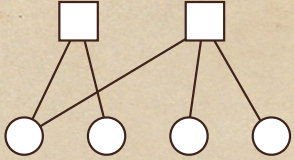
\includegraphics{Images/tanner_graph.png}}
  \caption{Tanner graph representation of a parity check matrix [2].}
  \label{fig}
\end{figure}

In Fig. \ref{fig}, we see that there are two check nodes, and four variable nodes.

A \textbf{cycle} in a Tanner graph is a closed path that starts and ends at the same node.

The \textbf{girth} of a Tanner graph is the length of the shortest cycle in the graph.
A larger girth is desirable because it leads to better error-correction performance.

A Tanner graph is useful for visualizing the relationship between parity check equations, in addition to acting as a visual mnemonic for certain LDPC decoding schemes.

\subsection{LDPC Parity Check and Generator Matrices}\label{matrices}
Given the parameters $(n,j,i)$, a valid LPDC parity check matrix may be constructed using the following procedure [2]:
\begin{enumerate}
  \item Construct a sub-matrix $H_0$ of dimensions $\frac{n-i}{j}$ by $n$, where a ``diagonal'' of $i$ ones is constructed.
    If we denote $1_1, 1_2, \ldots, 1_i$ as the ``indexed'' ones in each row, then the sub-matrix $H_0$ will look something like
    $$\begin{bmatrix}
      1_1   &\ldots& 1_i  & 0    & 0    & 0    & 0    &0     &\ldots& 0\\
      0     &\ldots& 0    & 1_1  &\ldots& 1_i  & 0    &0     &\ldots& 0\\
      \vdots&\ddots&\vdots&\vdots&\ddots&\vdots&\ddots&\vdots&\ddots&\vdots \\
      0     &\ldots& 0    & 0    &\ldots& 0    & 0    & 1_1  &\ldots& 1_i \\
    \end{bmatrix}$$
  \item Find $j - 1$ different matrices that have pseudo-random column permutations of $H_0$. Denote these new sub-matrices as $H_1, H_2, \ldots, H_{j-1}$.
  \item Construct the final parity check matrix $H$ by stacking sub-matrices $H_0,H_1,\ldots,H_{j-1}$ into a single $n-k$ by $n$ matrix.
\end{enumerate}

Given a parity check matrix $H$ for an LDPC code, the generator matrix $G$ can
be constructed.
If necessary, re-organize the codeword $\textbf{c}$ of length $n$ so that it is of the form $\textbf{c} = [\textbf{b}, \textbf{m}]$, where $\textbf{b}$ denotes the parity bits vector and $\textbf{m}$ denotes the message bits vector.
    We note that, if there are no errors in the codeword, then it must be that $\textbf{c}H^T = [\textbf{b}, \textbf{m}]H^T = 0$.

Sub-divide the parity matrix $H$ into two sub-matrices such that $H = [H_1, H_2]^T$ where $H_1$ is a square matrix of size $n-k$.
    Note that $\textbf{b}$ is of length $n-k$ as well.
    Therefore, we can break up the matrix
    multiplication into $[\textbf{b}, \textbf{m}][H_1, H_2]^T = \textbf{b}H_1^T + \textbf{m}H_2^T = 0$.
Since we are dealing with a code defined on a binary field, $\textbf{b}H_1^T = \textbf{m}H_2^T$ implies that $\textbf{b}= \textbf{m}H_2^T(H_1^T)^{-1}$.

    Let $A = H_2^T(H_1^T)^{-1}$, then the generator matrix $G$ is $[A, I_{n-k}]$.

\section{HDL Implementation of a Regular LDPC Code}
In order to assess the effectiveness of LDPC codes in memory, we implemented a sample LDPC code in System Verilog, a Hardware Description Language (HDL), which can be synthesized into logic gates and simulated on a Field-Programmable Gate Array (FPGA) board.

An interesting point that Gallager makes in Chapter III of his thesis [3] is the fact that the notion of an ``optimal'' $(j,i)$ is not well defined.
Gallager states that a regular LDPC code's limitation of capacity implies that the ``best'' $(j,i)$ code would perform essentially on the same level as a ``typical'', i.e. ``less optimal'' LDPC code with parameters $(j,i)$.
Consequently, when implementing an LDPC code in HDL, a convenient parity check matrix was selected.
In terms of hardware implementation, a sparse parity check matrix is more advantageous, since fewer gates could be used to implement the encoding and decoding logic.

We implemented an LDPC code parity matrix that had the same rate as 
the Hamming code we used for comparison.
Thus, we calculated that $R=\frac{k}{n}=\frac{64}{72}=1-\frac{8}{72} = \frac{j}{i}$.
To achieve this rate with the most sparse matrix, we worked with the LDPC code with parameters $n=72, j=2$ and $i=18$.

\subsection{Parity Check Matrix}
There are many possible parity check matrices for the above-mentioned parameters. The matrix we used for our implementation is included in our GitHub repository [1], since it is too large to be included in this report. The matrix was generated by a Python library called \href{https://hichamjanati.github.io/pyldpc/}{\texttt{pyldpc}} [4], using the procedure described in section \ref{matrices} of this report.

The following Python script was used to generate the parity check matrix:
\begin{verbatim}
import numpy as np
from pyldpc import make_ldpc

# parameters (n,j,i) = (72, 2, 18)
n = 72
d_v = 2
d_c = 18

H, G = make_ldpc(n, d_v, d_c, systematic=True)
\end{verbatim}

\subsection{Encoding}
The encoding was kept quite simple for this LDPC code.
The first 64 bits are interpreted as the message bits, and the last 8 bits are the parity bits.
The encoding is done by multiplying the message bits with the generator matrix, which can be constructed from the parity check matrix as described in section \ref{matrices}.
The encoding is done by multiplying the message bits with the generator matrix [7].
\subsection{Decoding}
For our HDL implementation, we used the bit-flipping decoding algorithm for LDPC codes.
To examine the resulting hardware, the RTL viewer can be found on the GitHub repository [1]. 
The decoding method uses a Tanner graph to visualize the structure of the LDPC code.
Furthermore, a recursive majority vote and bit flipping are used.

To summarize the algorithm in pseudo-code:
\begin{algorithm}
  \caption{Bit-Flipping Decoding Algorithm}
  \begin{algorithmic}
    \WHILE{parity check is not satisfied and maximum iteration is not reached}
      \FOR{each check node}
        \IF{the check node is not satisfied}
          \STATE vote for flipping the bit
        \ELSE
          \STATE{vote for not flipping the bit}
        \ENDIF
      \ENDFOR
      \STATE each bit vote for not flipping the bit
      \STATE flip the bit with the majority vote
    \ENDWHILE
    \IF {parity check is satisfied}
    \STATE return the decoded message
    \ELSE
    \STATE return failure
    \ENDIF
  \end{algorithmic}
\end{algorithm}

\subsection{Performance}
On DE1-SOC, Quartus analysis shows that the highest frequency it can run is \textbf{325.73 MHz} under \textit{slow 1100 mV 85C mode}. (Remark: It is a common analysis criteria to analyze the complexity of combinational logic path. It limits the maximum frequency of the circuit.)

Here is a smmary of resources usage and performance analysis by Quartus Prime:
% Looks like the table is too ugly, will do it manuuallly
% \begin{figure}[htbp]
%   \centerline{\includegraphics*{./Images/LDPC_resouce_usage.png}}
%   \caption{LDPC resource usage and performance analysis.}
%   \label{LDPC resource usage and performance analysis}
% \end{figure}
\begin{itemize}
  \item Combinational ALUT usage for logic: 114 \begin{itemize}
    \item 7 input functions: 0
    \item 6 input functions: 4
    \item 5 input functions: 10
    \item 4 input functions: 28
    \item $\leq$ 3 input functions: 72
  \end{itemize}
  \item Dedicated logic registers: 72
\end{itemize}

\section{Comparison with Hamming Code HDL Implementation}
Typical Hamming code implementation uses 64-bit to 72-bit encoding. Input is 64
bits since it is a typical cache line size. Although it is not an optimal
hamming code, it is a good visit pattern for computing systems.

This typical implementation is called \textbf{SECDED} (Single Error Correction,
Double Error Detection) Hamming code. It can detect and correct single-bit
errors and detect double-bit errors.

The concept of Hamming code is detecting errors in half of the codewords. And
then with different combinations of deleting patterns, we can locate a single
bit.

\begin{figure}[htbp]
  \centerline{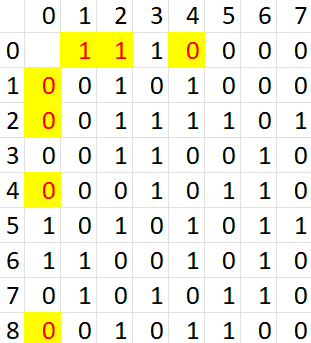
\includegraphics{Images/Hamming_example.png}}
  \caption{Parity bits and data bits in a Hamming code.}
  \label{fig_2}
\end{figure}

Since the output is more than 64 bits, we need 7 parity bits as shown in
\ref{fig_2}. For an interactive example, check out the Excel sheet in our
\href{https://github.com/luckunately/ELEC433-Projects}{GitHub Repo}[1]. %how can I add the reference hyperlink here?

The advantage of this kind of implementation would be that the difference of
parity bits is the coordinate of the error bit which makes it easier to find
the error bit.

We order the bits as shown below:

\begin{figure}[htbp]
  \centerline{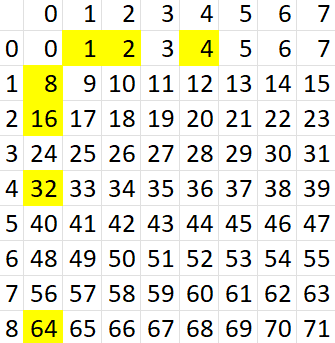
\includegraphics{Images/Hamming_bits_order.png}}
  \caption{Number parity bits and data bits in a Hamming code.}
  \label{fig_3}
\end{figure}

There are a total of 72 bits, which can be expressed in binary from
$6'b000\_0000$ to $6'b 100\_0111$. Note that there are exactly 7 bits which
corresponds to 7 parity bits. Mark the unique position vector as
\texttt{vec[6:0]} and let it be bijective to parity bits \texttt{p[6:0]}.

Now if we let $p0$ monitor all of the bits where the \texttt{vec[0]} is 1, $p1$
monitor all of the bits where the \texttt{vec[1]} is 1, and so on, we can find
the error bit by checking the parity bits. Note that the parity bit itself is
included in monitoring as well.

This way, if we calculate the parity bits and compare them with the received
parity bits, we can find the error bit. Since the parity bits are the
coordinate of the error bit, we can find the error bit by XORing the parity
bits.

\subsection{Implementation on FPGA}
% The typical cache-line size is 64 bits, thus we will use 64 bits input and one-bit error correction as the metrics to compare performance.
% \subsubsection{Hamming Implementation}

Because of the nature of the Hamming code, it is easier to implement on FPGA.
The error bit can be found by XORing the parity bits. The implementation can be
found in our \href{https://github.com/luckunately/ELEC433-Projects}{GitHub
  Repo}[1]. %how can I add the reference hyperlink here?

  RTL viewer can be found on GitHub for \href{https://github.com/luckunately/ELEC433-Projects/blob/add-tex/Hamming72out/Hamming72out_RTL.pdf}{Hamming72out} and \href{https://github.com/luckunately/ELEC433-Projects/blob/add-tex/Hamming64in/Hamming64inRTL.pdf}{Hamming64in}.

Although there are nearly 71 xor on a single combinational logic path, the time
delay is not significant. According to Quartus timing analysis, the highest
frequency it can run is \textbf{387.3 MHz} under \textit{slow 1100 mV 85C
  mode}.

Here is a summary of resources usage and performance analysis by Quartus Prime:
\begin{itemize}
  \item Combinational ALUT usage for logic: 154
  \begin{itemize}
    \item 7 input functions: 0
    \item 6 input functions: 121
    \item 5 input functions: 10
    \item 4 input functions: 13
    \item $\leq$ 3 input functions: 10
  \end{itemize}
  \item Dedicated logic registers: 69
\end{itemize}

% \subsubsection{Remarks on decoding}
% Encoding is relatively easy to implement. Just need to encode it with a series of XOR gates.

% However, decoding is more difficult. The decoding algorithm for the Hamming code is the \textbf{syndrome decoding} algorithm. The algorithm is as follows:

\section{Conclusion}
\textbf{TODO}

\begin{thebibliography}{00}
  \bibitem{b1} T. Wang and N. Balashov, ELEC433-Projects, 2024, GitHub repository, \url{https://github.com/luckunately/ELEC433-Projects}.
  \bibitem{b2} B. Kurkoski, Introduction to Low-Density Parity Check Codes, \url{https://www.jaist.ac.jp/~kurkoski/teaching/portfolio/uec_s05/S05-LDPC%20Lecture%201.pdf}.
  \bibitem{b3} R.G. Gallager, Low-Density Parity-Check Codes. Cambridge, MA: MIT Press, 1963 (Sc.D. MIT, 1960).
  \bibitem{b4} H. Janati, pyldpc, 2020, GitHub repository, \url{https://github.com/hichamjanati/pyldpc}.
  \bibitem{b5} B. Panzer-Steindel, Data integrity. CERN/IT, 2007, retrieved from \url{https://indico.cern.ch/event/13797/contributions/1362288/attachments/115080/163419/Data_integrity_v3.pdf}.
  \bibitem{b5}S. Jeon, E. Hwang, B. V. K. V. Kumar and M. K. Cheng, ``LDPC Codes for Memory Systems with Scrubbing'', 2010 IEEE Global Telecommunications Conference GLOBECOM 2010, Miami, FL, USA, 2010, pp. 1-6, doi: 10.1109/GLOCOM.2010.5683367.
  \bibitem{b6} S. Verma, S. Sharma, (2016) `FPGA implementation of low complexity LDPC iterative decoder', International Journal of Electronics, 103(7), pp. 1112-1126. doi:\url{https://doi.org/10.1080/00207217.2015.1087052}
\end{thebibliography}

\end{document}
